\subsection{机械波}

\begin{tabularx}{\columnwidth}{XX}
  波动通式      & $y=A\sin(\omega t\mp kx+\varphi_0)$，$k=\frac{2\pi}{\lambda}$ \\
  任意点振动方程  & $y=A\sin(\omega (t-\frac{x}{v})+\varphi_0)$ \\
  波速波长频率关系 & $v=\lambda f=\frac{\lambda}{T}$  \\
  相位差       & $\Delta\varphi=\frac{2\pi}{\lambda}\Delta x=2\pi\frac{\Delta t}{T}$ \\
  \multicolumn{2}{l}{\textbf{两波源在该点起振方向相同}} \\
  干涉加强条件   & $\Delta x=n\lambda$ \\
  干涉减弱条件   & $\Delta x=n\lambda+\frac12\lambda$  \\
  \multicolumn{2}{l}{\textbf{两波源在该点起振方向相反}} \\
  干涉加强条件   & $\Delta x=n\lambda+\frac12\lambda$ \\
  干涉减弱条件   & $\Delta x=n\lambda$ \\
  衍射条件     & 障碍尺寸越小、波长越大，衍射越明显。\\
  驻波条件     & 两列同频同振幅机械波相向传播\\
  多普勒效应    & 相互靠近频率变高；相互远离频率变低。\\
\end{tabularx}

\begin{formulanotebox}
\begin{itemize}[leftmargin=1.5em]
  \item 波速由介质决定，频率由振源决定；介质变化时优先判断频率是否不变。
  \item 写波动方程前先判断传播方向；沿 $+x$ 方向传播常写成 $y=A\sin(\omega t-kx+\varphi_0)$。
  \item 干涉增强/减弱判定要先看“起振方向同相或反相”，再代波程差条件。
  \item 同侧法判断振动方向时，振动方向与传播方向在波形图同一侧。
\end{itemize}
\end{formulanotebox}

\begin{keypointbox}
\begin{itemize}[leftmargin=1.5em]
  \item 机械波大题常见三步：写方程、找相位差、定增强减弱。
  \item 双曲线法和同心等距圆法是双波源干涉图像判定的两种标准工具。
\end{itemize}
\end{keypointbox}

\begin{center}
  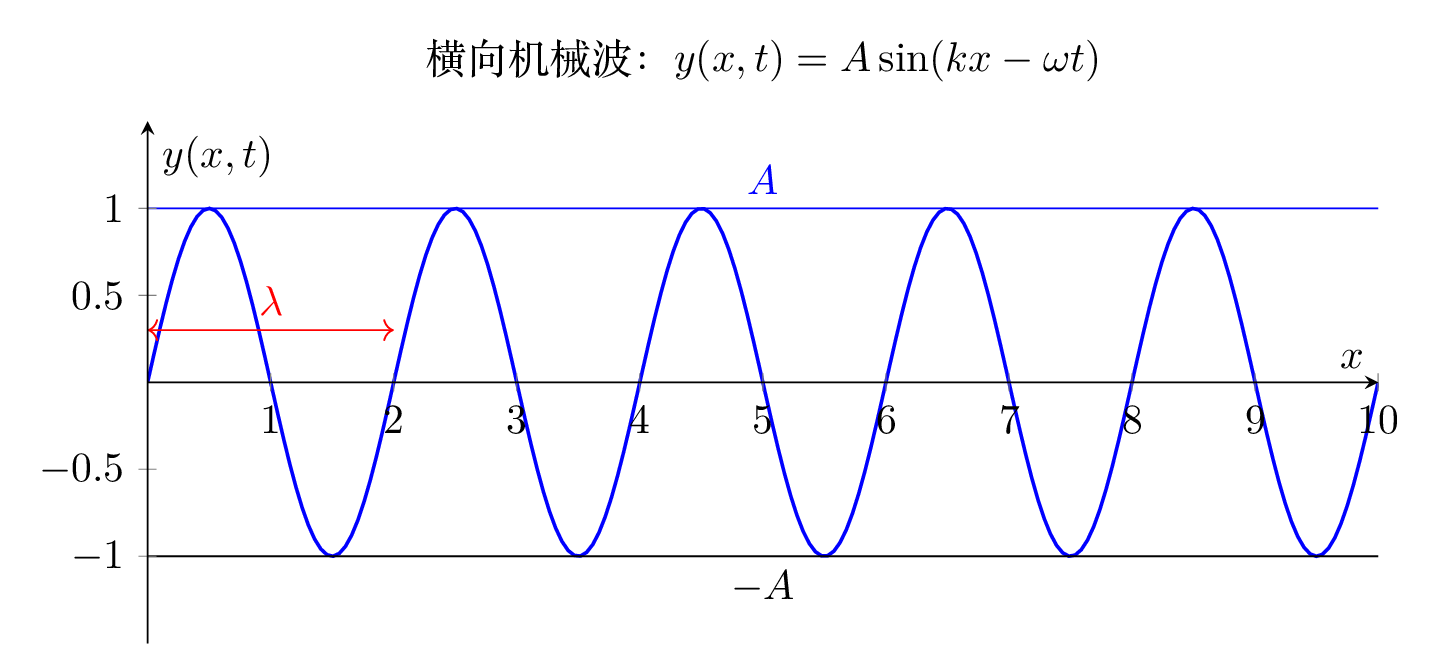
\includegraphics[width=0.82\columnwidth]{../assets/wave_profile.png}

  \vspace{4pt}
  {\small 横波波形与波长示意}
\end{center}

\begin{center}
  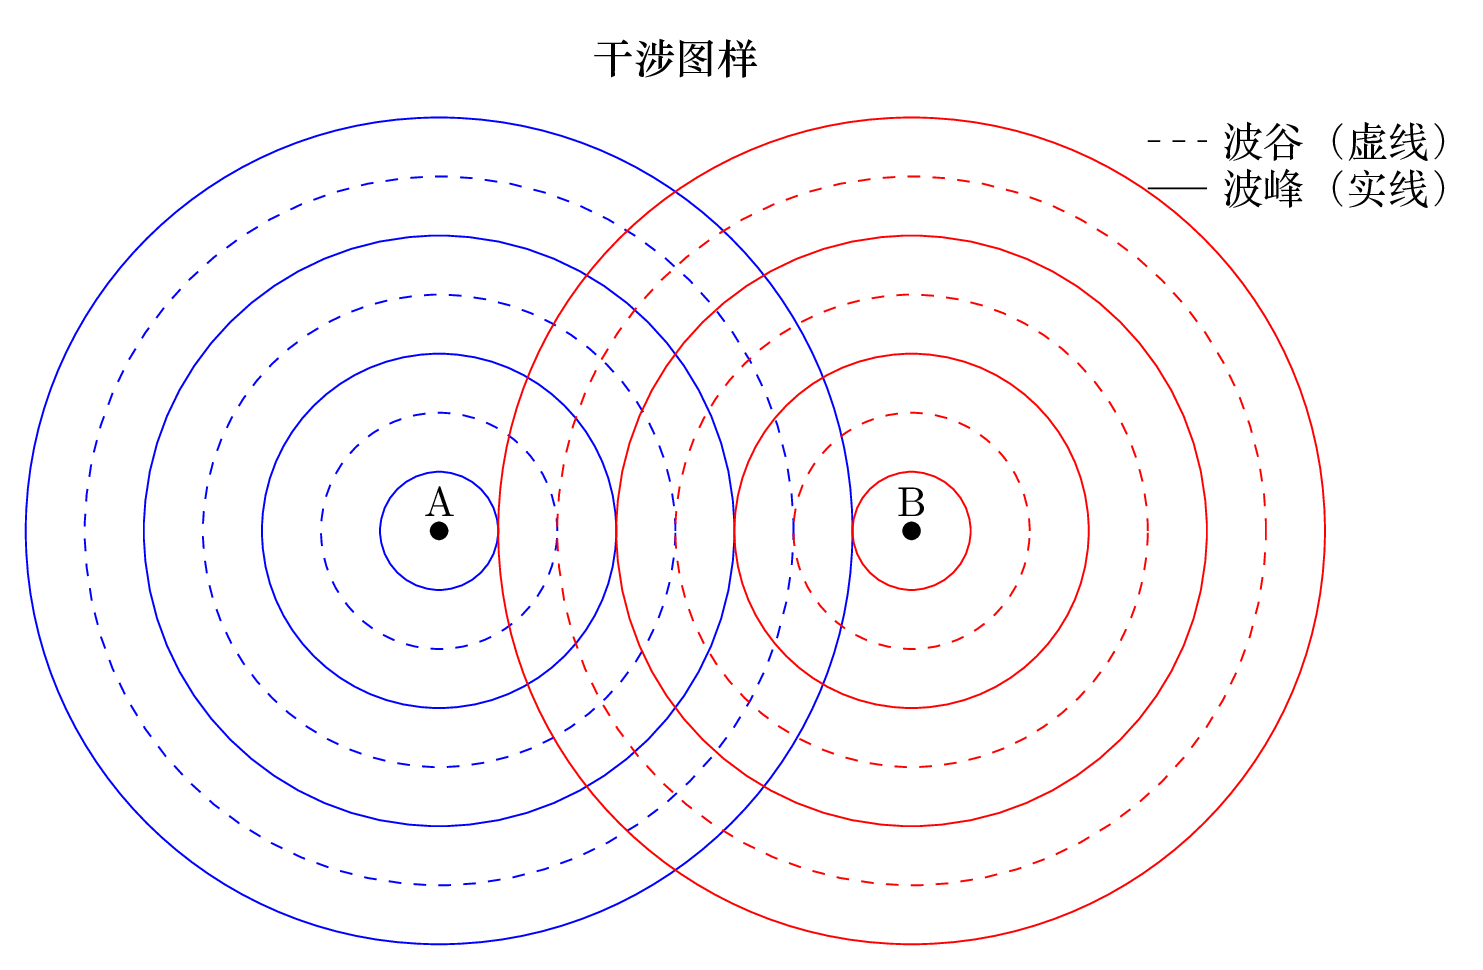
\includegraphics[width=0.72\columnwidth]{../assets/wave_interference_circles.png}

  \vspace{4pt}
  {\small 双波源同心等距圆干涉示意}
\end{center}

\begin{center}
  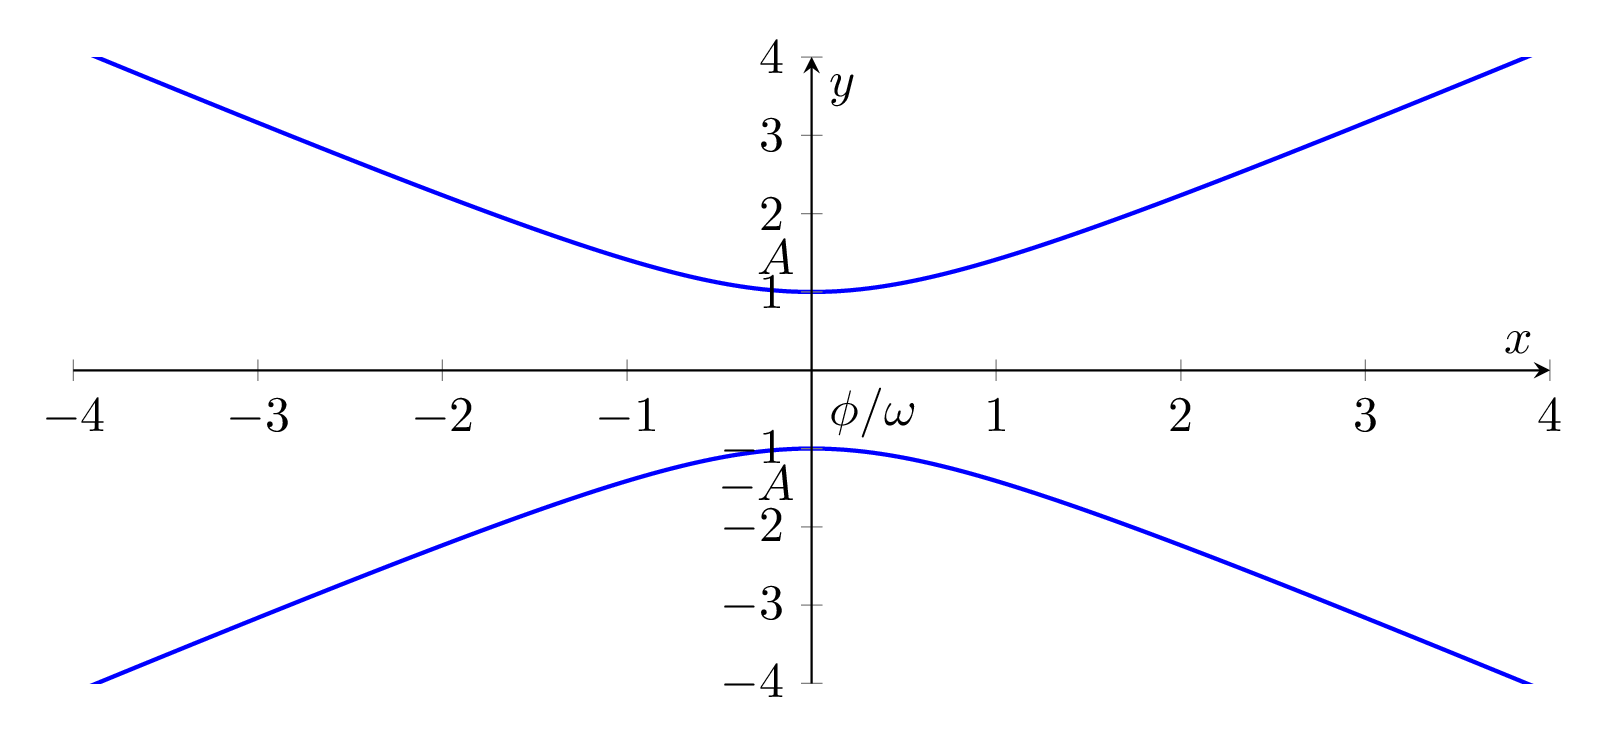
\includegraphics[width=0.72\columnwidth]{../assets/wave_interference_hyperbola.png}

  \vspace{4pt}
  {\small 干涉双曲线边界示意}
\end{center}

\begin{casetypebox}[title={\strut\textcolor{white}{\bfseries 常见题型：干涉图样判定}}]
\begin{itemize}[leftmargin=1.5em]
  \item 先算到两波源的波程差 $\Delta x=|r_1-r_2|$，再结合两波源起振方向判断加强或减弱。
  \item 两波源同相时，加强点满足 $\Delta x=n\lambda$，减弱点满足 $\Delta x=(n+\frac12)\lambda$。
  \item 两波源反相时，加强和减弱条件互换。
  \item 图像判定可用同心等距圆找波峰、波谷，也可用双曲线表示波程差相同的点。
\end{itemize}
\end{casetypebox}

\begin{casetypebox}[title={\strut\textcolor{white}{\bfseries 常见题型：波动图像与振动图像}}]
\begin{itemize}[leftmargin=1.5em]
  \item 波形图是某一时刻不同位置质点的位移，振动图像是某一质点在不同时刻的位移。
  \item 已知传播方向判断质点振动方向，可用“微小平移法”：把波形沿传播方向稍微平移，质点下一瞬间的位置变化就是振动方向。
  \item 由图读出 $\lambda$、$T$ 后，用 $v=\frac{\lambda}{T}$ 求波速；同一介质中波速不随振幅改变。
\end{itemize}
\end{casetypebox}
